% Author: Izaak Neutelings (April 2021)
% Derivation by Ondřej Sedláček (November 2022)
\documentclass[border=3pt,tikz]{standalone}
\usepackage{amsmath}
\usepackage{physics}
\usepackage{siunitx}
\usepackage{xcolor}
\usepackage{etoolbox} %ifthen
\usepackage[outline]{contour} % glow around text
\usetikzlibrary{angles,quotes,arrows.meta} % for pic
\contourlength{1.0pt}

\colorlet{myblue}{blue!70!black}
\colorlet{mydarkblue}{blue!40!black}
\colorlet{mygreen}{green!50!black}
\colorlet{myred}{red!65!black}
\colorlet{xcol}{blue!85!black}
\colorlet{vcol}{green!70!black}
\colorlet{projcol}{vcol!90!black!60}
\tikzstyle{wave}=[myblue,thick]
\tikzstyle{xline}=[very thick,myblue]
\tikzstyle{vline}=[very thick,mygreen]
\tikzstyle{vector}=[->,very thick,vcol,line cap=round]
\tikzstyle{mydashed}=[green!30!black!90,dash pattern=on 2pt off 2pt,very thin]
\tikzstyle{mymeas}=[{Latex[length=3,width=2]}-{Latex[length=3,width=2]},thin]
\def\tick#1#2{\draw[thick] (#1) ++ (#2:0.05*\ymax) --++ (#2-180:0.1*\ymax)}


\begin{document}

% TRAJECTORY - PARABOLA + breakdown
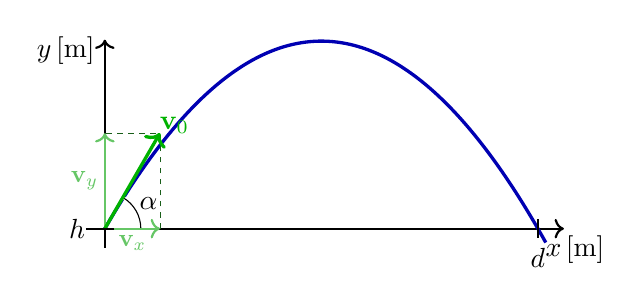
\begin{tikzpicture}
  \def\v{1.4}
  \def\xmax{5.5}
  \def\ymax{2.4}
  \def\ang{60}
  \def\d{(\xmax)} % distance landing point
  \def\b{tan(\ang)} % slope at x=0
  \def\h{0} % height h
  \def\a{-((\b*\d+\h)/\d^2)} % coefficient
  \def\nsamples{100}
  \def\vx{{\v*cos(\ang)}}
  \def\vy{{\v*sin(\ang)}}
  \coordinate (O) at (0,\h);
  \coordinate (Vx) at ({\v*cos(\ang)},\h);
  \coordinate (Vy) at (0,{\h+\v*sin(\ang)});
  \coordinate (V) at ({\v*cos(\ang)},{\h+\v*sin(\ang)});
  
  % AXES & TRAJECTORY
  \draw[->,thick]
    (-0.1*\ymax,0) -- (1.06*\xmax,0) node[right=4,below=-1] {$x$\,[m]};
  \draw[->,thick]
    (0,-0.1*\ymax) -- (0,\ymax) node[below=4,left=0] {$y$\,[m]};
  \draw[xline,variable=\t,samples=\nsamples,smooth,domain=0:\d+0.1]
    plot(\t,{\a*\t^2+\b*\t+\h}); %node[right=7,above=-2] {$x=x(t)$};
  
  % VELOCITY VECTOR
  \draw pic["\contour{white}{$\alpha$}",draw=white,double=black,double distance=0.4,
            angle radius=13,angle eccentricity=1.4] {angle = Vx--O--V};
  \draw[mydashed]
    (Vx) |- (Vy);
  \draw[<->,projcol,thick]
    (Vy) -- (O) node[scale=0.9,midway,left=-1] {$\vb{v}_y$}
      -- (Vx) node[scale=0.9,midway,below=-1] {$\vb{v}_x$};
  \draw[->,vcol,very thick,line cap=round]
    (O) --++ ({\ang}:\v) node[above right=-4] {$\vb{v}_0$};
  \tick{O}{0} node[left] {$h$};
  \tick{{\d},0}{90} node[below] {$d$};
  
\end{tikzpicture}



\end{document}
